\section{Overall Design}
\label{sec:design}

\begin{figure}[!t]
	\center
	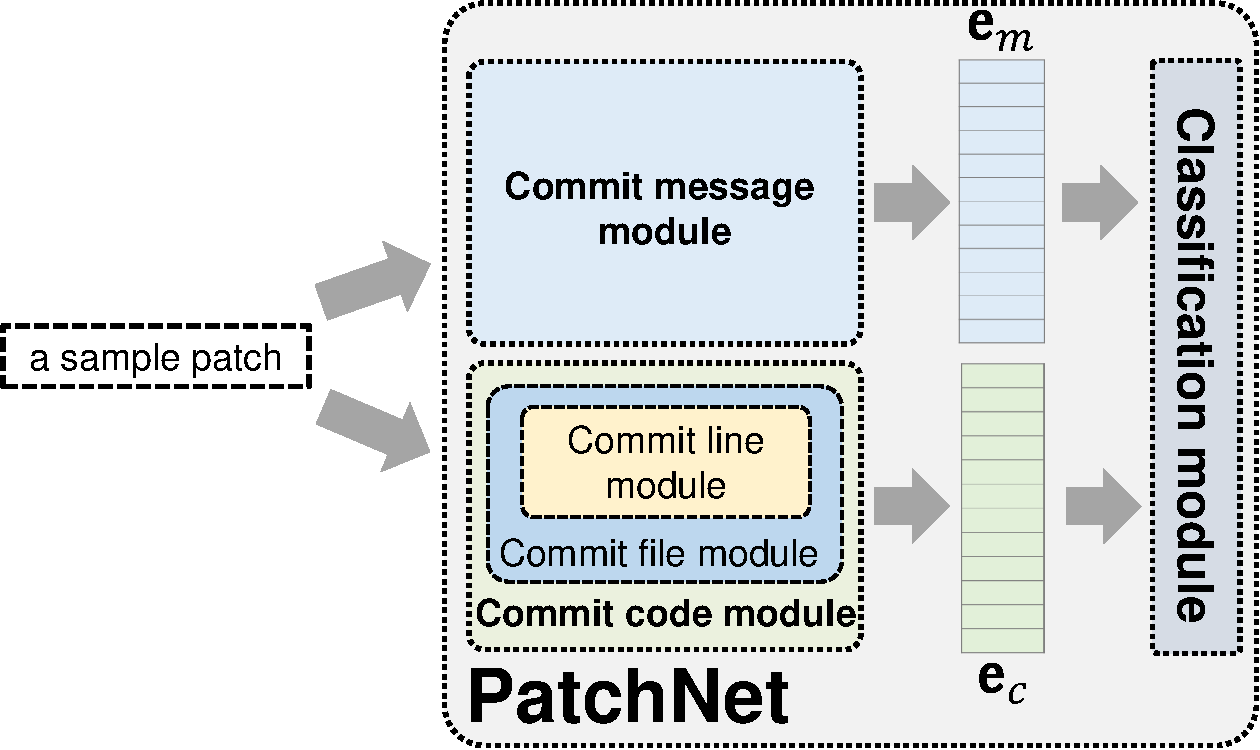
\includegraphics[scale=0.38]{figures/overall_patchnet.pdf}
	\caption{The proposed PatchNet framework. $\textbf{e}_m$ and $\textbf{e}_c$ are embedding vectors collected from the commit message module and commit code module respectively.}
	\label{fig:patchnet}
    \vspace{-0.4cm}
\end{figure}

Figure~\ref{fig:patchnet} shows an overall framework of our PatchNet. Our tool accepts as input a set of patches, which contain both commit messages and commit code. The output of PatchNet is a list of predicted scores that reflects how likely the given patches are bug fixing patches. Our framework includes three main modules: the \textit{commit message module}, the \textit{commit code module}, and the \textit{classification module}.